\documentclass[letterpaper, 12pt]{report}
\usepackage[utf8]{inputenc}
\usepackage[english, spanish]{babel}
\usepackage{fullpage} 
\usepackage{graphicx}
\usepackage{enumitem}
\usepackage{chngcntr}
\usepackage{float}
\usepackage{hyperref} 
\counterwithin{figure}{section}
\renewcommand{\thesection}{\arabic{section}}
\renewcommand{\thesubsection}{\thesection.\arabic{subsection}}
\renewcommand{\baselinestretch}{1.5}
\begin{document}

\begin{titlepage}
	\centering
	
\includegraphics[width=0.3\textwidth]{eii_ulpgc.png}\par\vspace{1cm}
	{\scshape\LARGE Universidad de Las Palmas de Gran Canaria \par}
	\vspace{1cm}
	{\scshape\Large Programaci\'on de Aplicaciones M\'oviles Nativas \par}
	\vspace{.2cm}
    {\scshape\Large Accesibilidad y normativa. Análisis de aplicaciones. \par}
	\vspace{1cm}
	{\Large\bfseries Informe sobre accesibilidad\par}
	\vspace{1cm}
	{\itshape Paula Rosa Rodríguez Morales \par}
	\vfill

	\vfill
	{\large \today\par}
\end{titlepage}

\begin{abstract}
En este informe se evalúa la accesibilidad de un sitio web y de una aplicación móvil, siguiendo las pautas WCAG. Se analiza el cumplimiento de los principios de Perceptibilidad, Operabilidad, Comprensibilidad y Robustez en ambos casos.
\end{abstract}

\tableofcontents
\newpage

\section{Ejercicio 1: Evaluación de accesibilidad de un sitio web}

En este ejercicio, se nos solicita seleccionar un sitio web y realizar una evaluación de su accesibilidad conforme a las pautas WCAG. Para este caso, he escogido el sitio web de Amazon España, \url{https://www.amazon.es}. El objetivo es analizar el cumplimiento de las pautas que aseguran que el contenido digital sea accesible para personas con diversas discapacidades.

La accesibilidad web se fundamenta en cuatro principios clave que deben cumplirse para garantizar una experiencia inclusiva. Estos principios son:
\begin{itemize}
    \item Perceptible
    \item Operable
    \item Comprensible
    \item Robusto
\end{itemize}

Para llevar a cabo esta evaluación, primero utilizamos pruebas manuales para identificar aquellos problemas que no pueden ser detectados únicamente con herramientas automáticas. 

\subsection{Perceptibilidad}

Uno de los aspectos más importantes en la perceptibilidad es asegurarse de que todos los elementos visuales, como las imágenes, estén acompañados de un texto alternativo que describa su contenido. El texto alternativo es crucial para que las personas que usan lectores de pantalla puedan comprender la función o el significado de la imagen sin verla.

Para realizar esta verificación, abrimos las herramientas de desarrollador en el navegador, utilizando la tecla F12, seleccionamos una imagen y revisamos el atributo alt para cada una de ellas.

En el caso de Amazon España, hemos encontrado que las imágenes importantes, como las que representan productos o promociones, sí contienen descripciones adecuadas en el atributo alt. Esto lo podemos observar claramente en las Figuras \ref{fig:1} y \ref{fig:2}, donde los comentarios en el atributo alt describen de manera precisa el contenido de las imágenes.

\begin{figure}[H]
\centering
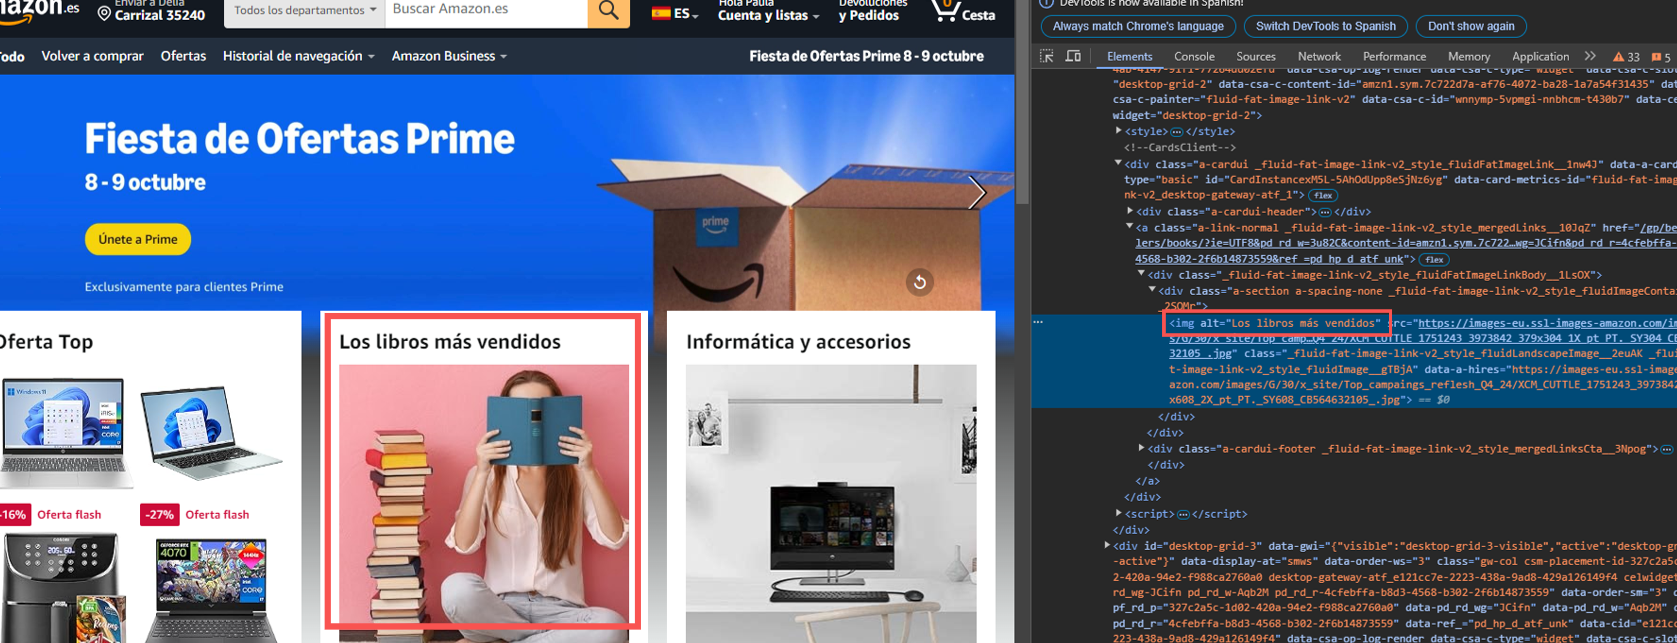
\includegraphics[width=1\textwidth]{figure1.png}
\caption{Imagen con texto que incluye una descripción del objeto representado.}
\label{fig:1}
\end{figure}

\begin{figure}[H]
\centering
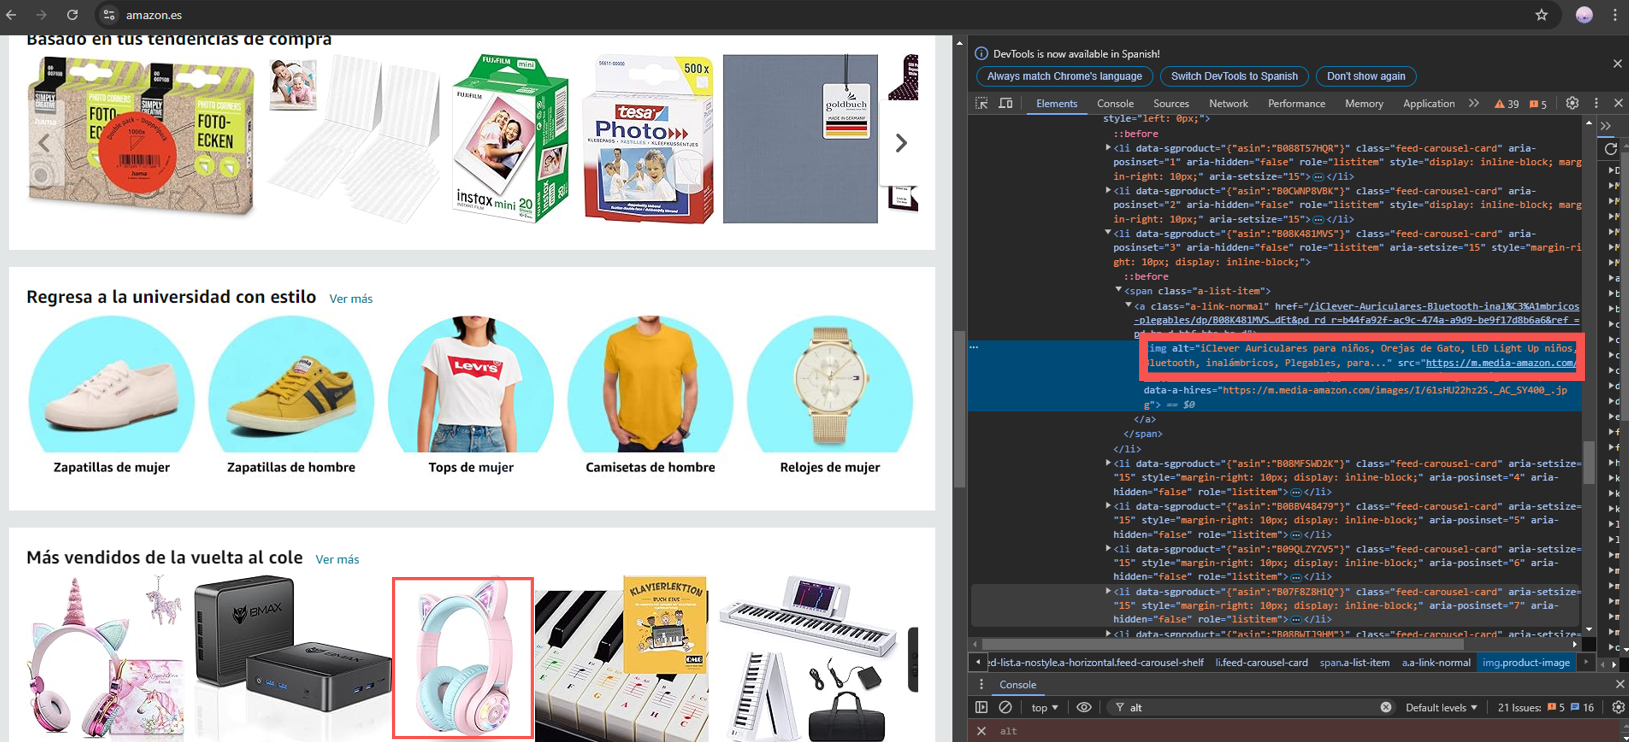
\includegraphics[width=1\textwidth]{figure2.png}
\caption{Atributo alt con comentario descriptivo.}
\label{fig:2}
\end{figure}

No obstante, no todas las imágenes deben contener texto alternativo. En algunos casos, existen imágenes decorativas cuyo único propósito es estético y que no aportan información relevante. Estas imágenes deben tener un atributo alt vacío (es decir, alt=""), como es el caso de la flecha que indica la opción de volver a reproducir, visible en la Figura \ref{fig:3}. En la Figura \ref{fig:4}, observamos que este principio se ha cumplido adecuadamente, ya que la flecha no aporta información significativa y, por lo tanto, su atributo alt está vacío.

\begin{figure}[H]
\centering
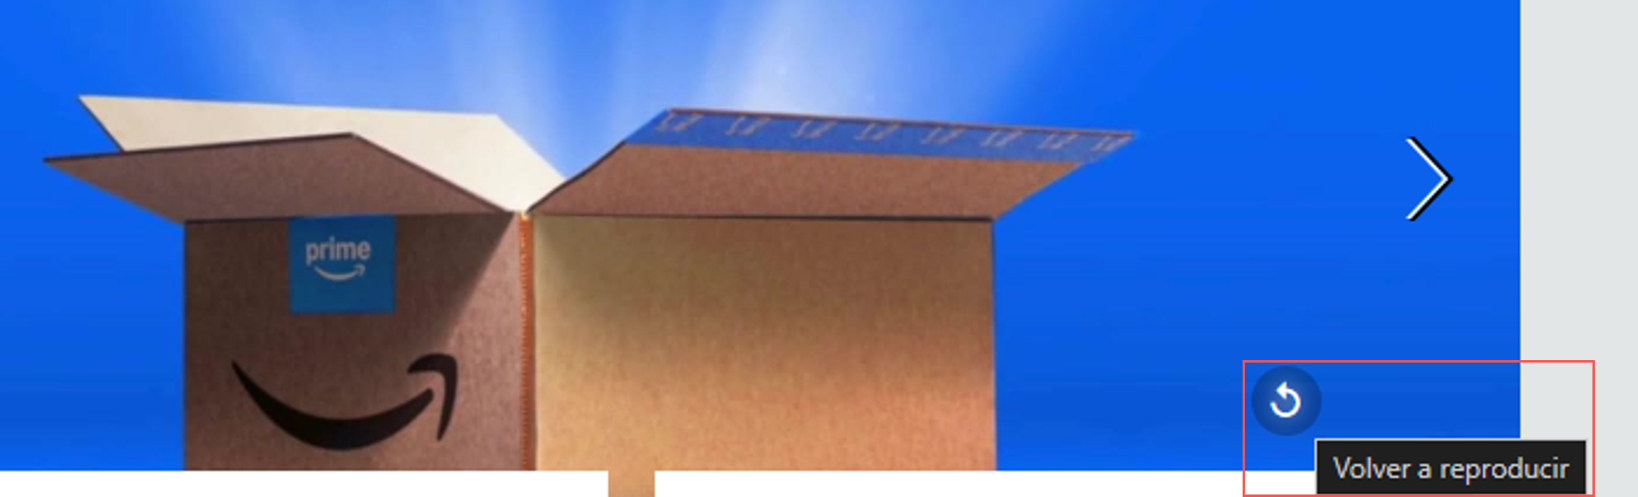
\includegraphics[width=1\textwidth]{figure3.png}
\caption{Flecha volver a reproducir.}
\label{fig:3}
\end{figure}

\begin{figure}[H]
\centering
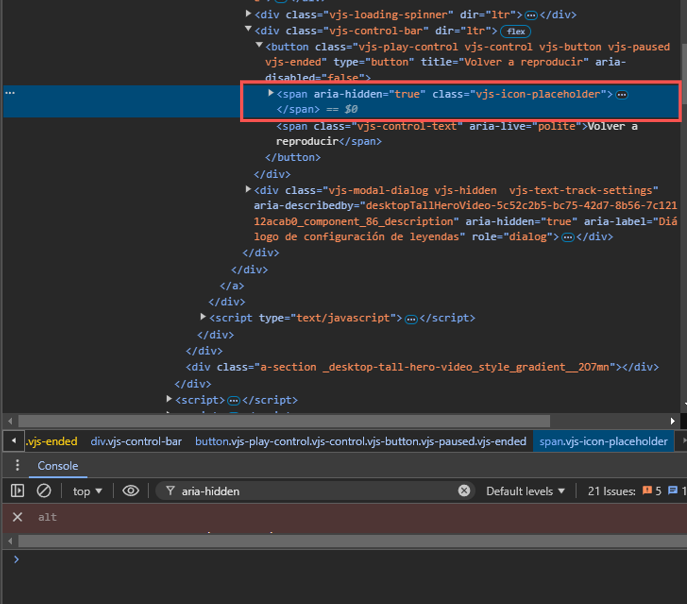
\includegraphics[width=0.7\textwidth]{figure4.png}
\caption{Atributo alt vacío en imagen decorativa.}
\label{fig:4}
\end{figure}

Sin embargo, encontramos excepciones. En la Figura \ref{fig:5}, una imagen de la película ``John Wick 4'' cuenta con el atributo aria-hidden, lo que oculta la imagen de los lectores de pantalla. Considero que esto es un error, ya que la imagen podría interesar a los usuarios. Eliminar el aria-hidden o proporcionar un alt descriptivo en este caso mejoraría la accesibilidad.

\begin{figure}[H]
\centering
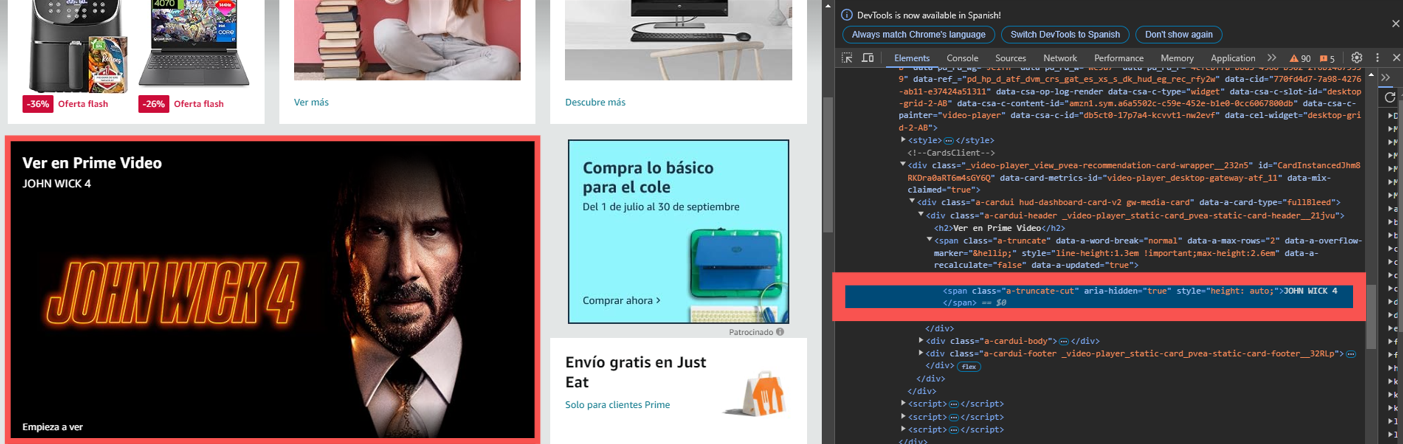
\includegraphics[width=1\textwidth]{figure5.png}
\caption{Aria-hidden detectado en una imagen que debería poseer atributo alt descriptivo.}
\label{fig:5}
\end{figure}

Otro aspecto clave de la perceptibilidad son los subtítulos en los vídeos. Para verificar este punto, reproducimos varios vídeos disponibles en el sitio web y analizamos si cuentan con subtítulos. En el vídeo mostrado en la Figura \ref{fig:6}, comprobamos que los subtítulos están presentes, son exactos y están sincronizados con el contenido hablado. ¿Este hecho se puede observar cuando en una escena donde se pronuncia la palabra ``Who?'' en inglés, los subtítulos lo traducen correctamente al español como ``¿Quién?'', como se ve en la Figura \ref{fig:7}.

\begin{figure}[H]
\centering
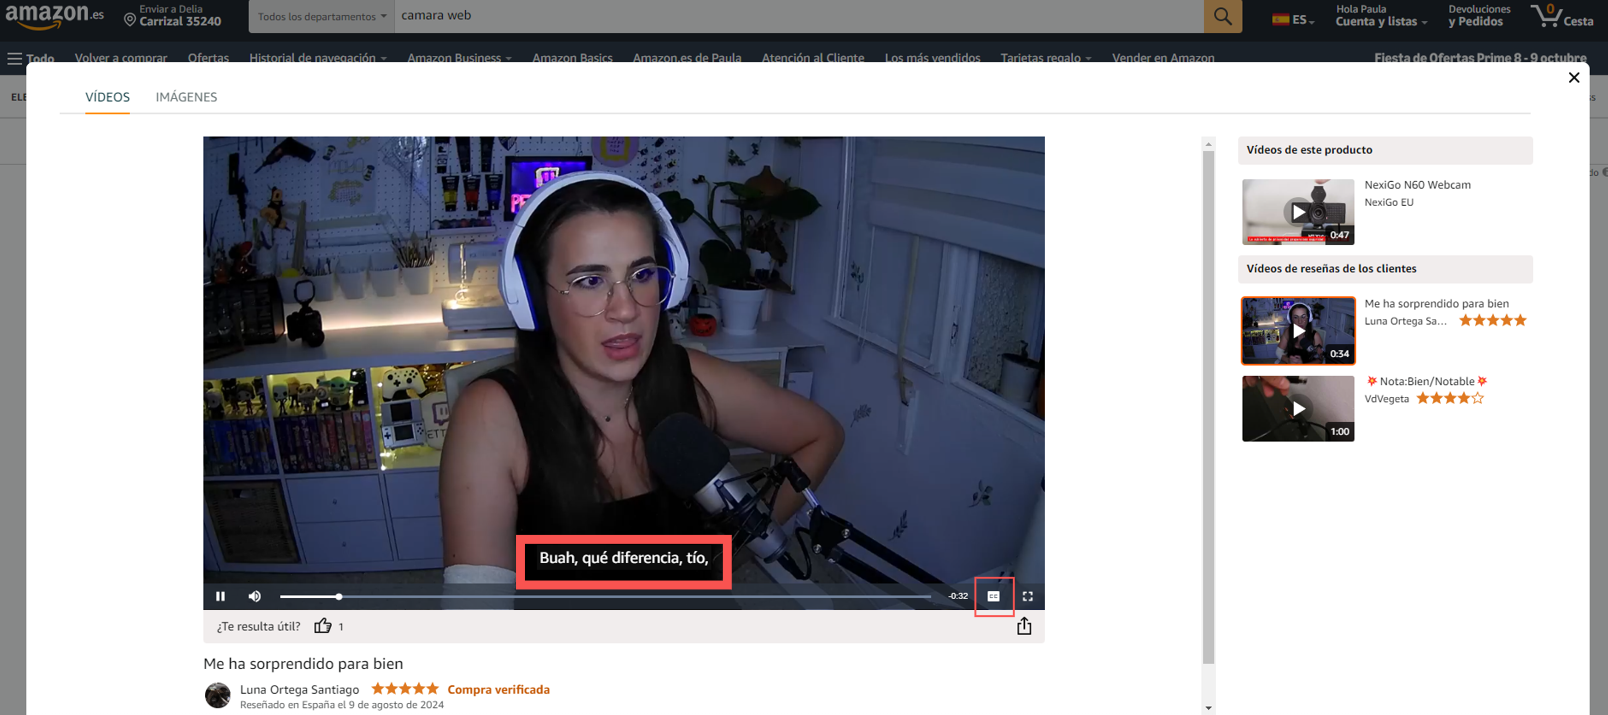
\includegraphics[width=1\textwidth]{figure6.png}
\caption{Subtítulos presentes correctamente en un vídeo.}
\label{fig:6}
\end{figure}

\begin{figure}[H]
\centering
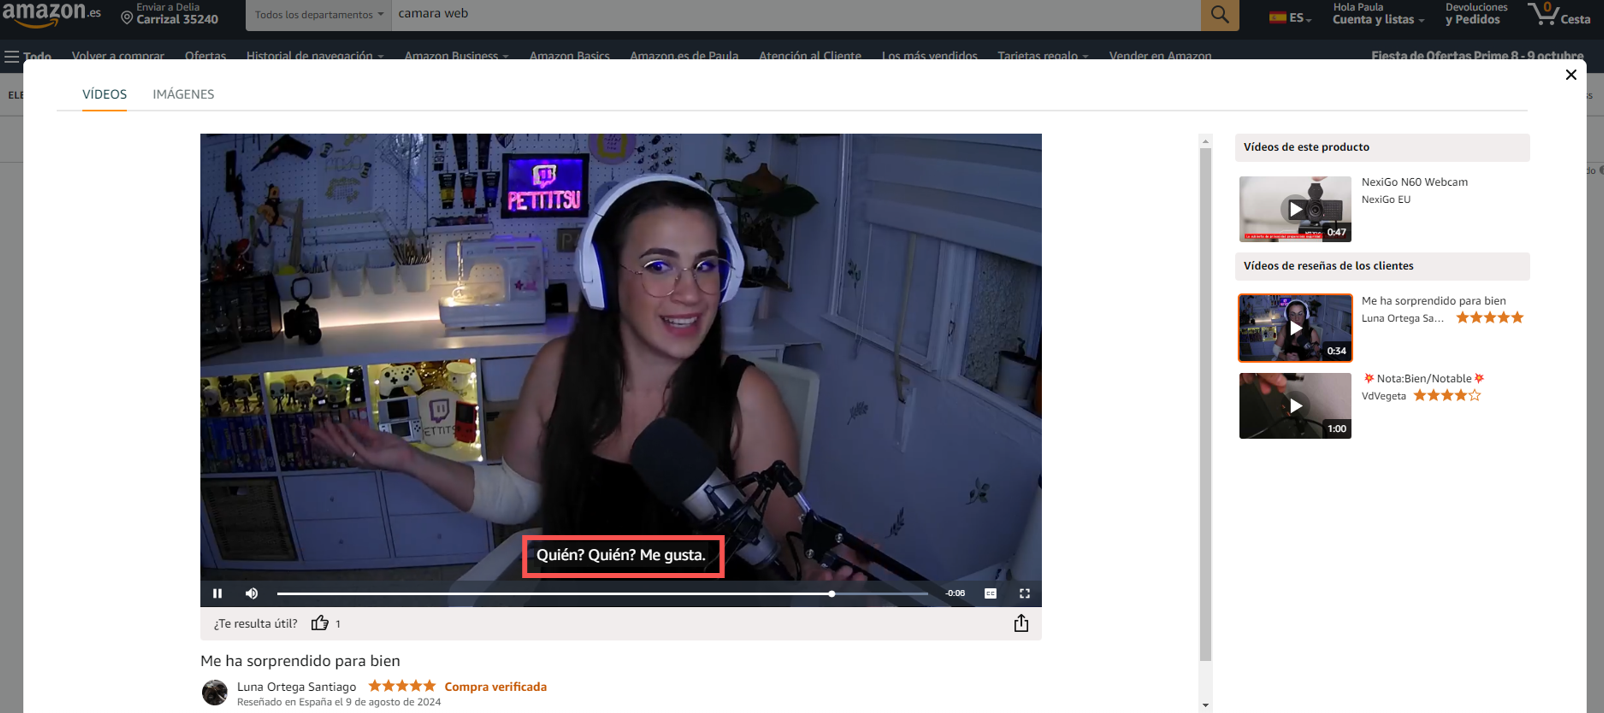
\includegraphics[width=1\textwidth]{figure7.png}
\caption{Subtítulos bien traducidos al idioma deseado.}
\label{fig:7}
\end{figure}

No obstante, en otro vídeo, representado en la Figura \ref{fig:8}, no existe la opción de activar subtítulos ni transcripciones, lo que supone un punto negativo para la accesibilidad del sitio. Esto es especialmente importante para personas con dificultades auditivas que dependen de los subtítulos para comprender el contenido de los vídeos o para personas que no pueden reproducir el audio, por ejemplo, porque se encuentran en una biblioteca y no disponen de auriculares.

\begin{figure}[H]
\centering
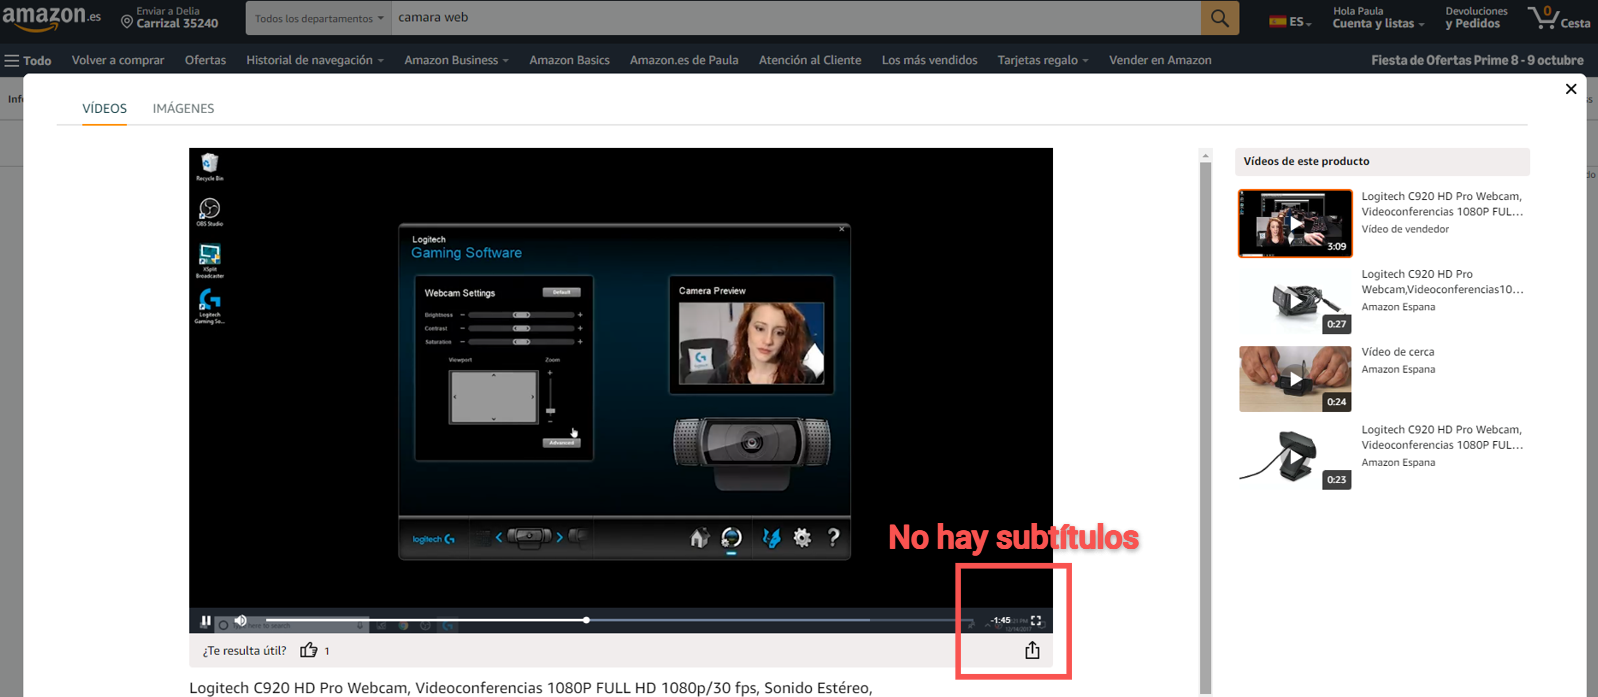
\includegraphics[width=1\textwidth]{figure8.png}
\caption{Video sin subtítulos ni transcripciones.}
\label{fig:8}
\end{figure}

También es necesario revisar el contraste del texto con el fondo para garantizar que sea lo suficientemente alto como para facilitar su lectura, algo que parece correcto a simple vista, aunque más adelante en este informe se analizará de forma más precisa mediante herramientas especializadas.

Además, evaluaremos la adaptabilidad del sitio al redimensionar la ventana del navegador. Hasta ahora, hemos comprobado que el sitio funciona bien a una escala del 100\%. Al redimensionarlo al 50\% (como se muestra en la Figura \ref{fig:9}) y al 200\% (ver Figura \ref{fig:10}), hemos observado que en la vista al 50\%, todos los elementos siguen siendo visibles. Sin embargo, al aumentar al 200\%, algunos elementos se extienden fuera del área visible, lo que requiere desplazamiento horizontal. A pesar de esto, es positivo que los elementos no se superpongan, manteniendo el diseño legible y funcional.

\begin{figure}[H]
\centering
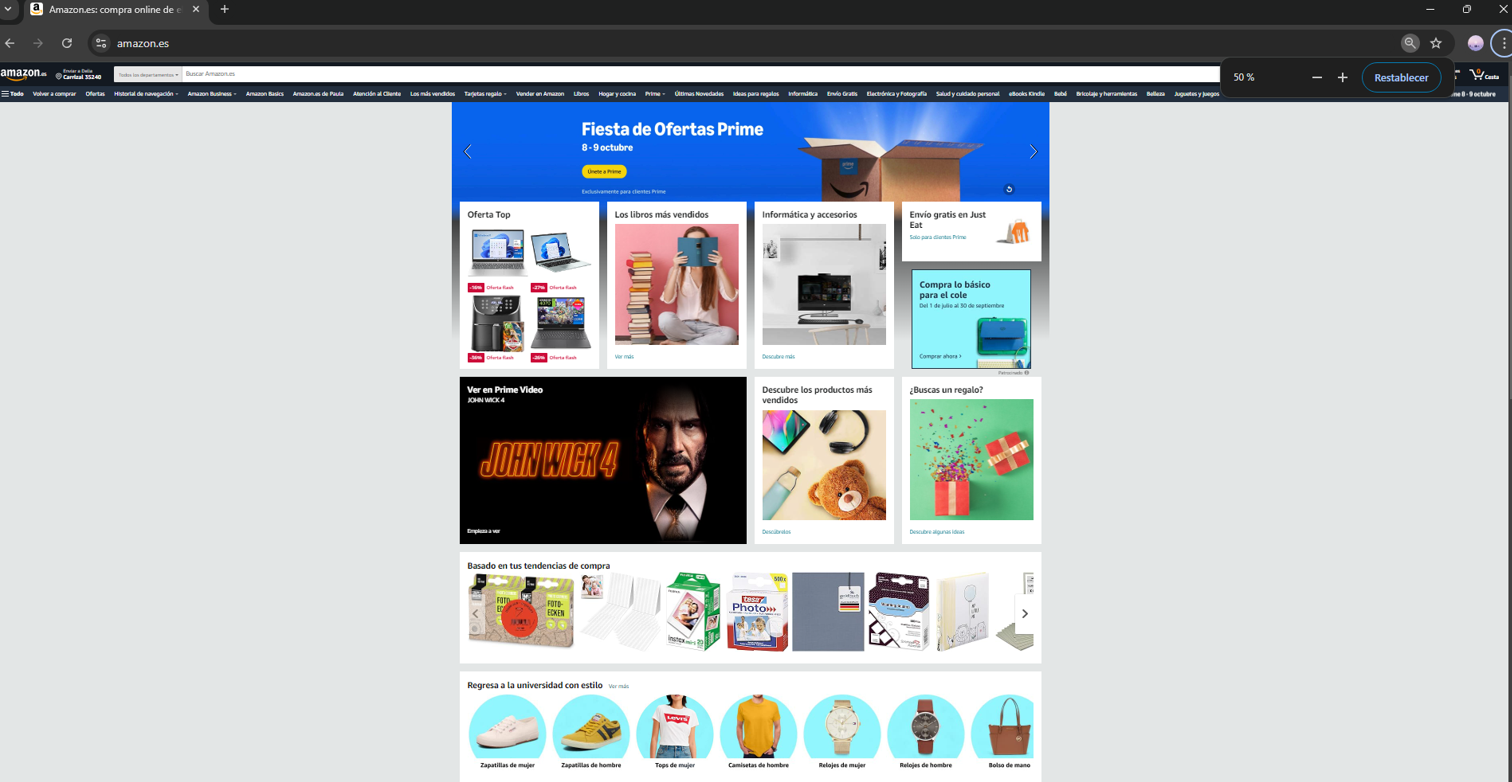
\includegraphics[width=1\textwidth]{figure9.png}
\caption{Página web redimensionada al 50\%.}
\label{fig:9}
\end{figure}

\begin{figure}[H]
\centering
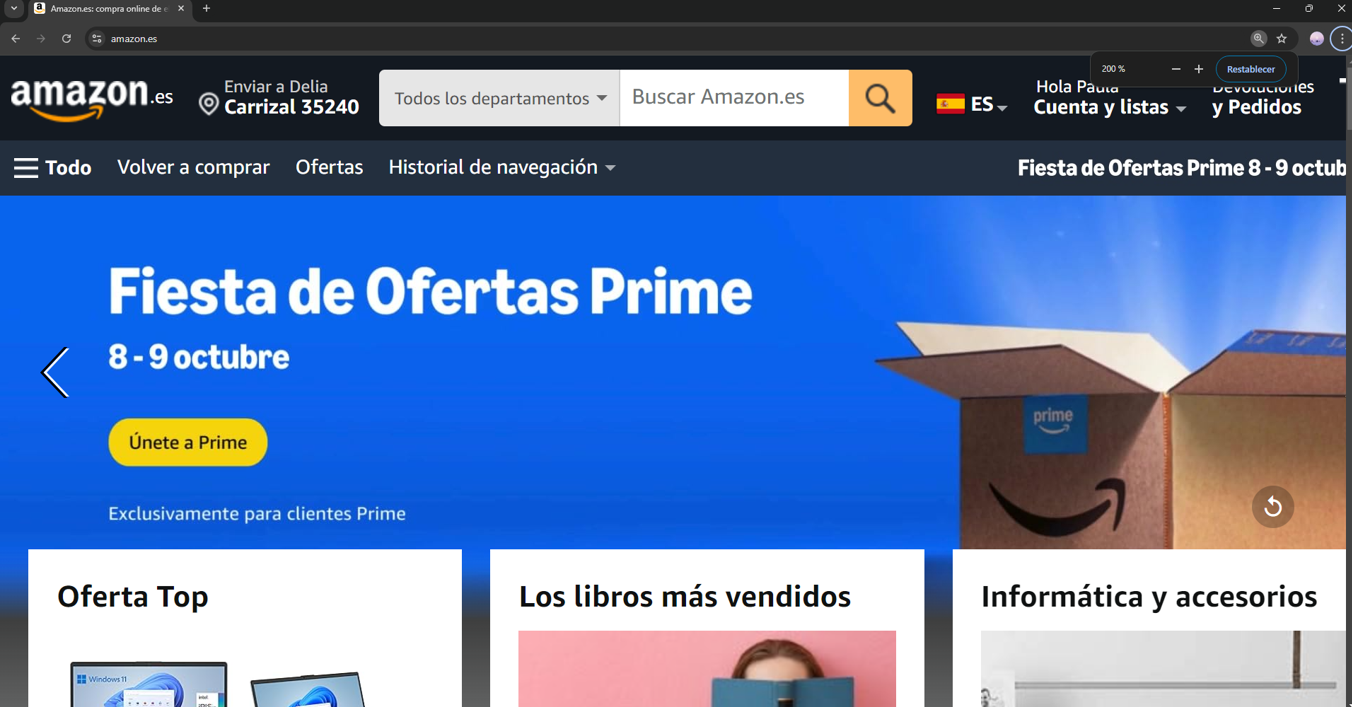
\includegraphics[width=1\textwidth]{figure10.png}
\caption{Página web redimensionada al 200\%.}
\label{fig:10}
\end{figure}

Además, observamos en la Figura \ref{fig:11}, que el comportamiento del sitio web en dispositivos móviles es igual.

\begin{figure}[H]
\centering
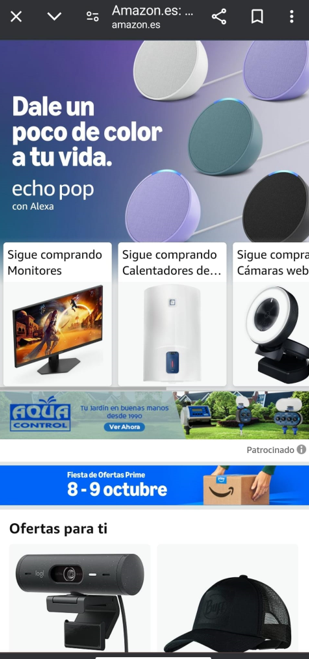
\includegraphics[width=0.5\textwidth]{figure11.png}
\caption{Comportamiento de la web accediendo desde teléfono móvil.}
\label{fig:11}
\end{figure}

\subsection{Operabilidad}

Para comprobar la operabilidad del sitio, nos aseguraremos de que la navegación sea completamente funcional usando solo el teclado, lo cual es crucial para usuarios que no pueden usar un ratón. Hemos comprobado, como se muestra en las Figuras \ref{fig:12} y \ref{fig:13}, que la navegación por teclado es posible utilizando combinaciones como Shift+Tab, enter y la barra espaciadora, siendo el enfoque claramente visible.

\begin{figure}[H]
\centering
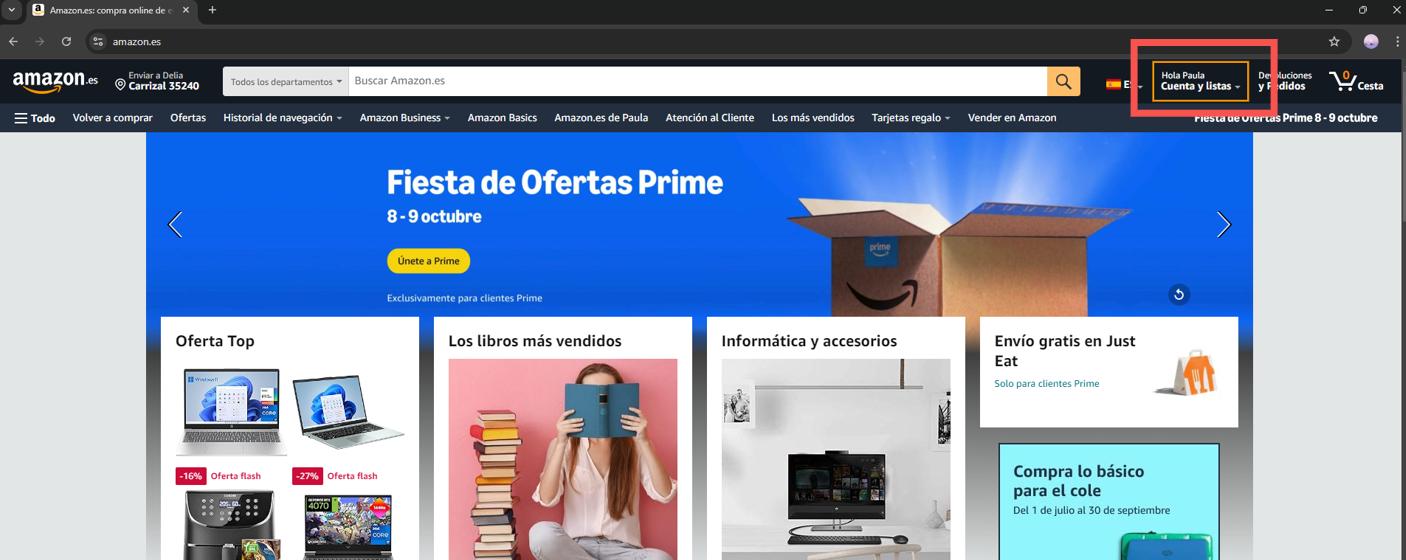
\includegraphics[width=1\textwidth]{figure12.png}
\caption{Utilización del teclado para navegar por la web.}
\label{fig:12}
\end{figure}

\begin{figure}[H]
\centering
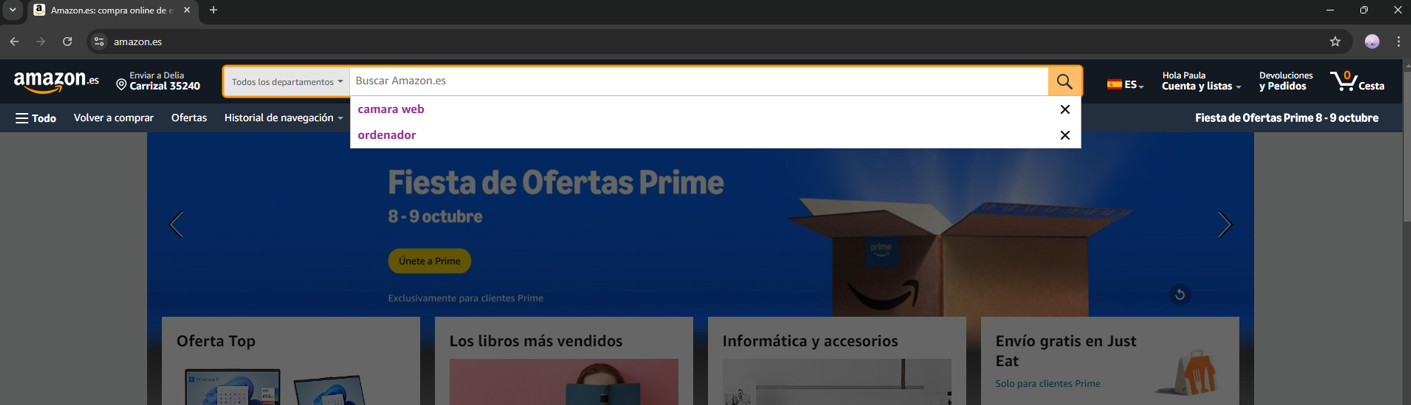
\includegraphics[width=1\textwidth]{figure13.png}
\caption{Utilización del teclado para navegar por la web.}
\label{fig:13}
\end{figure}

Al navegar por la web utilizando solo el teclado, observamos que los enlaces y botones son accesibles, y su tamaño es adecuado para que puedan ser seleccionados con facilidad. Los botones corresponden, en muchos casos, a imágenes de productos, las cuales, al ser de tamaño grande y claramente visibles, facilitan su selección. Sin embargo, detectamos que los titulares de los productos son relativamente pequeños en comparación con las imágenes. Esto podría ser una complicación para usuarios con visión reducida, por lo que sería recomendable aumentar el tamaño de estos textos.

Otro aspecto de la operabilidad es el tiempo disponible para interactuar con los elementos en pantalla. En Amazon España, observamos que los usuarios no tienen un tiempo limitado para interactuar con los sliders de productos, ya que estos son manuales y no se desplazan automáticamente. Esto permite que el usuario tenga tiempo suficiente para leer y usar el contenido, lo cual es especialmente importante para personas con discapacidades cognitivas. Además, como se puede ver en la Figura \ref{fig:14}, el proceso de compra tampoco tiene un límite de tiempo para ser completado.

\begin{figure}[H]
\centering
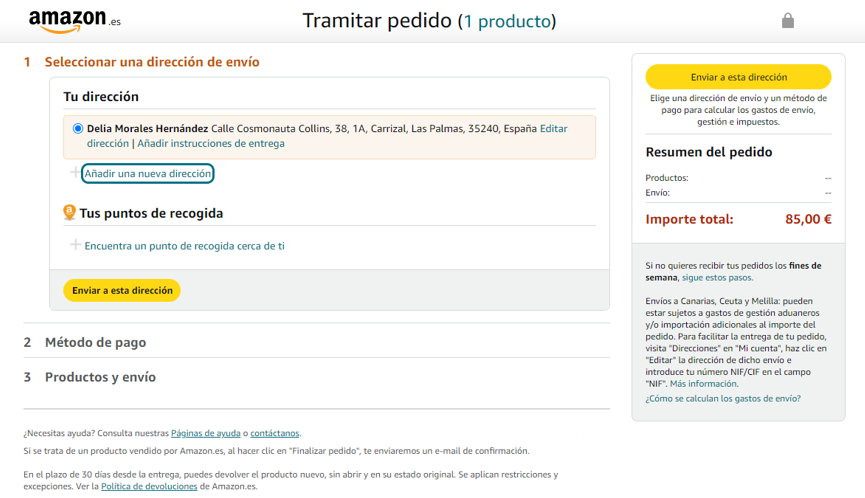
\includegraphics[width=1\textwidth]{figure14.png}
\caption{Proceso de compra sin tiempo límite.}
\label{fig:14}
\end{figure}

\subsection{Comprensibilidad}

El siguiente principio para evaluar es la comprensibilidad. Este aspecto está relacionado con la facilidad con la que los usuarios pueden entender tanto el contenido del sitio web como la manera en que está estructurado. Durante nuestra evaluación, verificamos que el lenguaje utilizado en el sitio web es claro y conciso, evitando tecnicismos innecesarios que podrían dificultar la comprensión del contenido.

Para evaluar la estructura del contenido, hemos inspeccionado los encabezados y subencabezados del sitio, revisando el uso de etiquetas como \texttt{<h1>}, \texttt{<h2>}, \texttt{<h3>}, etc. En la Figura \ref{fig:15}, se muestra un encabezado de nivel H2 que hemos podido identificar en la vista del controlador del navegador.

\begin{figure}[H]
\centering
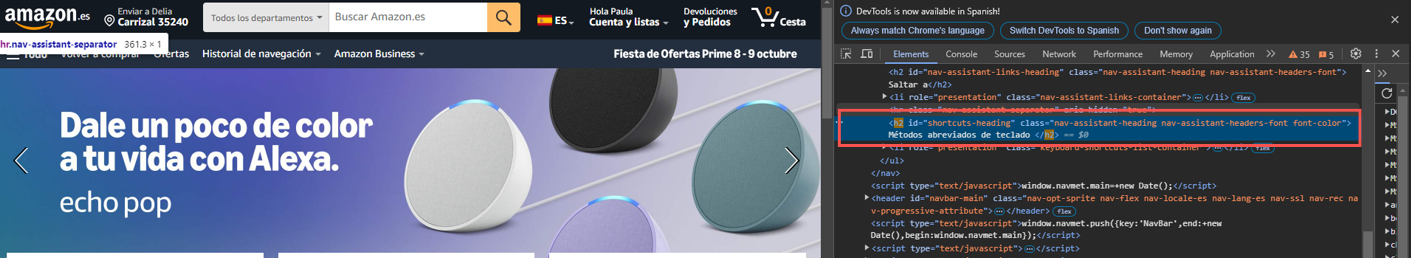
\includegraphics[width=1\textwidth]{figure15.png}
\caption{Encabezado h2 en vista de controlador.}
\label{fig:15}
\end{figure}

Sin embargo, durante esta revisión, encontramos algunos problemas relacionados con la jerarquía de encabezados. Por ejemplo, en algunas partes del sitio, se salta directamente de un \texttt{<h1>} a un \texttt{<h4>}, sin utilizar encabezados intermedios como \texttt{<h2>} o \texttt{<h3>}. Esto puede confundir a las tecnologías de asistencia que dependen de esta estructura para navegar por la página.

Otro punto que considerar en este aspecto es la facilidad con la que los usuarios pueden detectar y corregir errores en los formularios. En la Figura \ref{fig:16}, mostramos un formulario que detecta y señala errores de entrada de manera clara, proporcionando sugerencias útiles para que los usuarios puedan corregir dichos errores.

\begin{figure}[H]
\centering
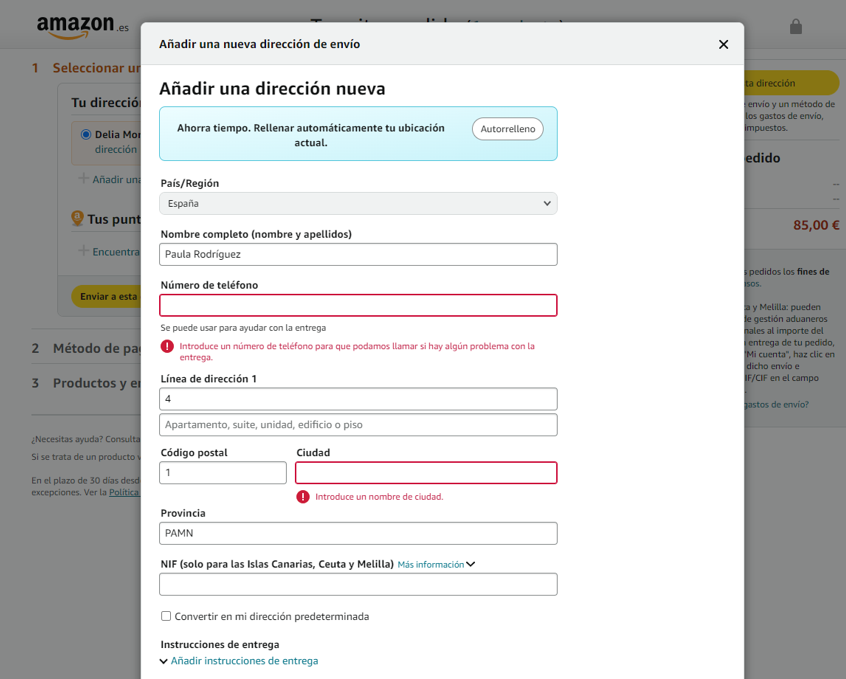
\includegraphics[width=1\textwidth]{figure16.png}
\caption{Formulario con detección de argumentos incorrectos.}
\label{fig:16}
\end{figure}

Además, es importante destacar el uso de banderas como método de selección de idioma, como lo hace Amazon.es. Aunque visualmente pueden ayudar a algunos usuarios a asociar un idioma con un país de manera rápida, este enfoque tiene limitaciones. Por ejemplo, no todos los hablantes de un idioma se identifican con una sola bandera. El uso de la bandera de España para representar el español, o de la bandera del Reino Unido para el inglés, puede excluir a los hablantes de otras regiones que comparten el mismo idioma, por lo que sería recomendable acompañar las banderas con texto alternativo que indique claramente el idioma, o incluso mejor, ofrecer un menú de texto desplegable y prescindir de las banderas.

\subsection{Robustez}

Por último, analizamos la robustez del sitio web. Para comprobamos si el sitio web funciona bien en diferentes navegadores. Durante la evaluación inicial, utilizamos el navegador Google Chrome y observamos que el sitio funcionaba correctamente. Para asegurarnos de que esta robustez se mantenga en otros entornos, probamos el sitio en Microsoft Edge, tal como se muestra en la Figura \ref{fig:17}, y comprobamos que el rendimiento del sitio es igualmente bueno.

\begin{figure}[H]
\centering
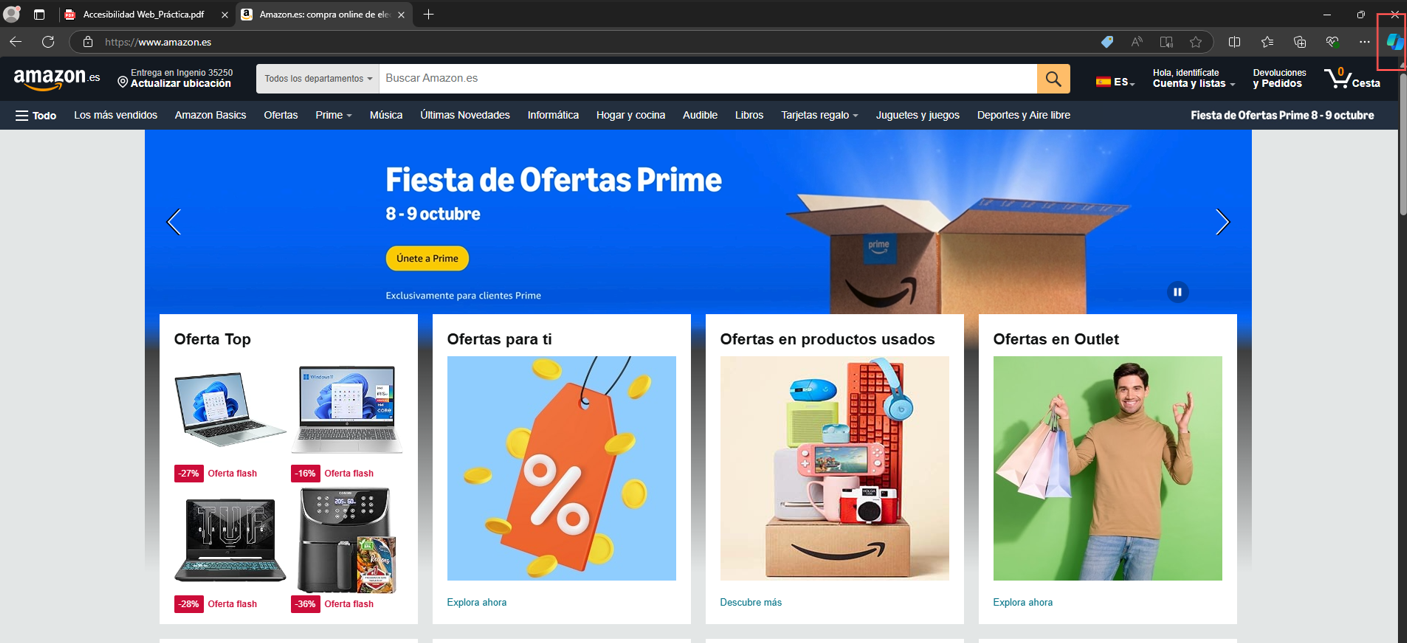
\includegraphics[width=1\textwidth]{figure17.png}
\caption{Acceso a la web desde el navegador Microsoft Edge.}
\label{fig:17}
\end{figure}

\subsection{Uso de herramientas automáticas}

Para obtener un análisis más detallado y preciso, empleamos varias herramientas automáticas que nos permiten identificar problemas de accesibilidad que podrían no ser visibles a simple vista. La primera herramienta que utilizamos es la WAVE Web Accessibility Evaluation Tool \url{https://wave.webaim.org}, una plataforma que permite examinar la accesibilidad de una página web en profundidad. Como se muestra en la Figura \ref{fig:18}, esta herramienta nos indica errores de accesibilidad relacionados con texto alternativo faltante, así como problemas de bajo contraste que no detectamos manualmente.

\begin{figure}[H]
\centering
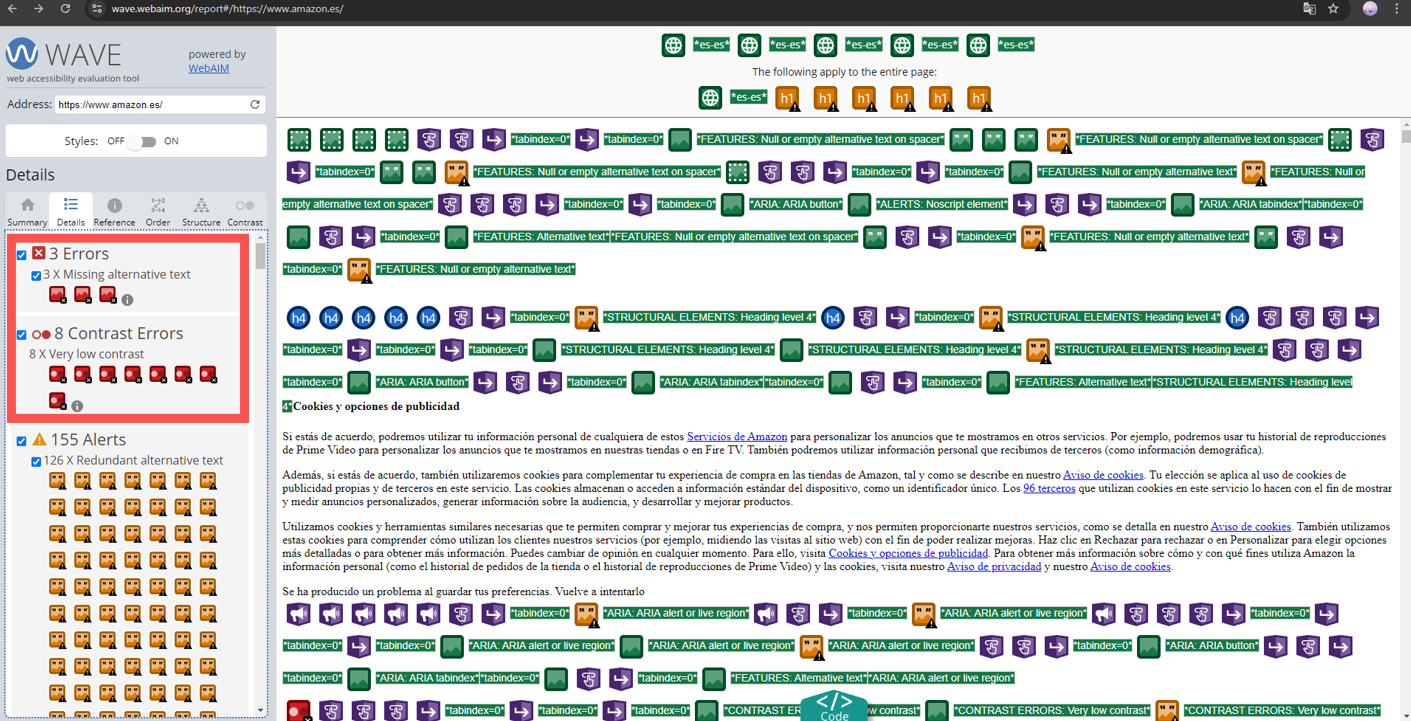
\includegraphics[width=1\textwidth]{figure18.png}
\caption{Examinación de la web mediante WAVE Web Accessibility Evaluation Tool.}
\label{fig:18}
\end{figure}

Debido a los problemas de contraste que identificamos, decidimos emplear una herramienta adicional, el SCAG Color Contrast Checker \url{https://chrome.google.com/webstore/detail/wcag-color-contrast-check/plnahcmalebffmaghcpcmpaciebdhgdf?hl=en}. Esta herramienta permite medir las relaciones de contraste entre el texto y el fondo para asegurar que cumplen con los estándares mínimos establecidos por las pautas WCAG. Como se observa en la Figura \ref{fig:18}, las relaciones de contraste en su mayoría son adecuadas, pero en algunas zonas del sitio, el contraste es insuficiente. Para texto normal, el contraste debe ser al menos de 4.5:1, mientras que para texto grande el valor mínimo es de 3:1.

\begin{figure}[H]
\centering
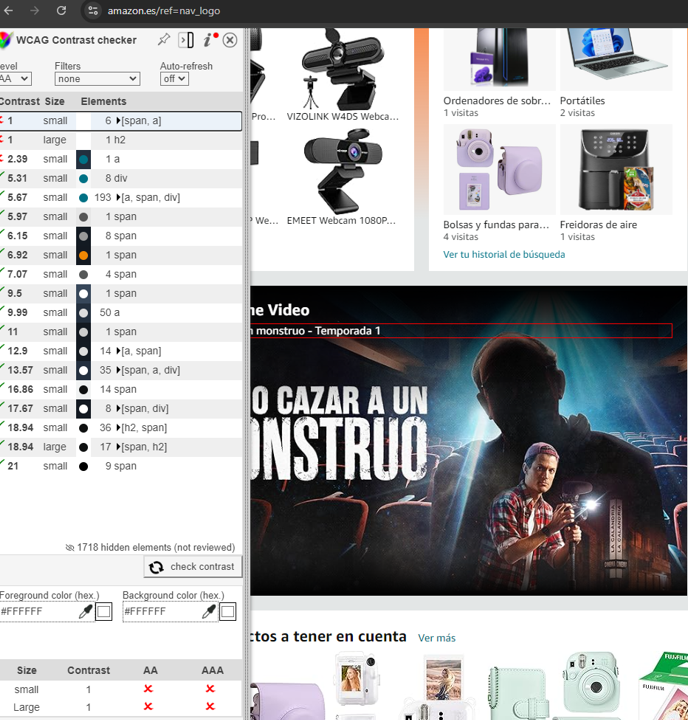
\includegraphics[width=1\textwidth]{figure19.png}
\caption{Comprobación del contraste de la web usando SCAG Color contrast checker.}
\label{fig:19}
\end{figure}

Además de las herramientas mencionadas, también empleamos Google Lighthouse, una herramienta integrada en Google Chrome que proporciona un análisis de la accesibilidad de un sitio web. Para usar esta herramienta, accedimos a la opción Lighthouse dentro de las herramientas para desarrolladores de Chrome, tal como se muestra en la Figura \ref{fig:19}.

\begin{figure}[H]
\centering
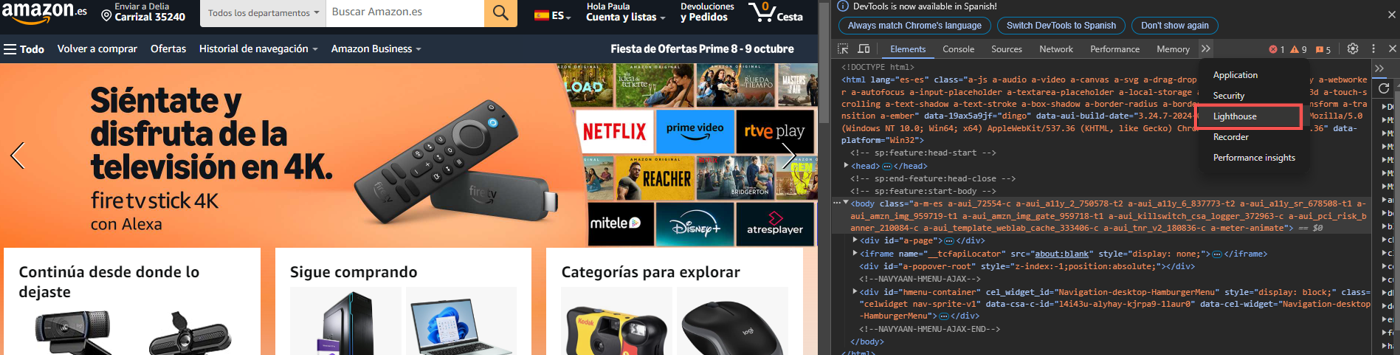
\includegraphics[width=1\textwidth]{figure20.png}
\caption{Pestaña lighthouse desde las herramientas para desarrolladores de Chrome.}
\label{fig:20}
\end{figure}

Una vez dentro, seleccionamos el tipo de dispositivo en el que nos encontramos, así como lo que queremos analizar, que en este caso es únicamente la accesibilidad.

\begin{figure}[H]
\centering
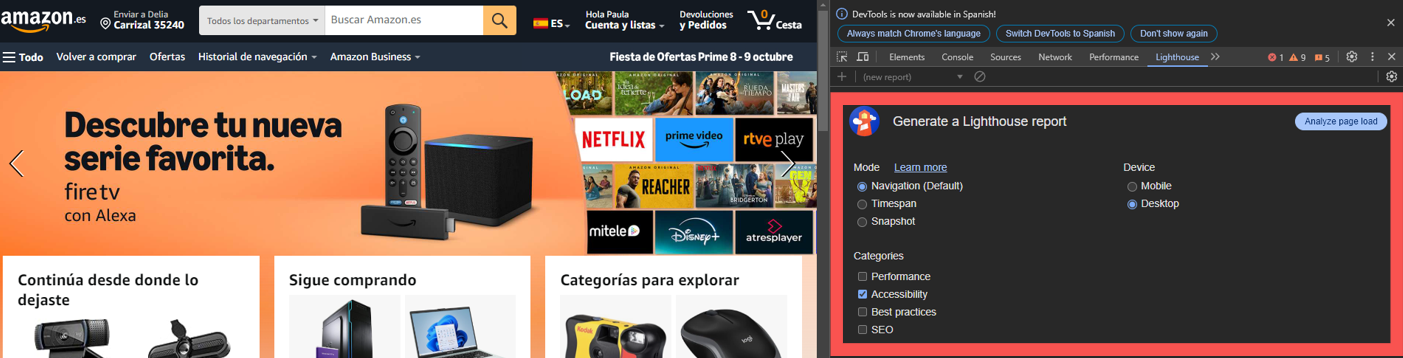
\includegraphics[width=1\textwidth]{figure21.png}
\caption{Generación de informe desde lighthouse.}
\label{fig:21}
\end{figure}

\begin{figure}[H]
\centering
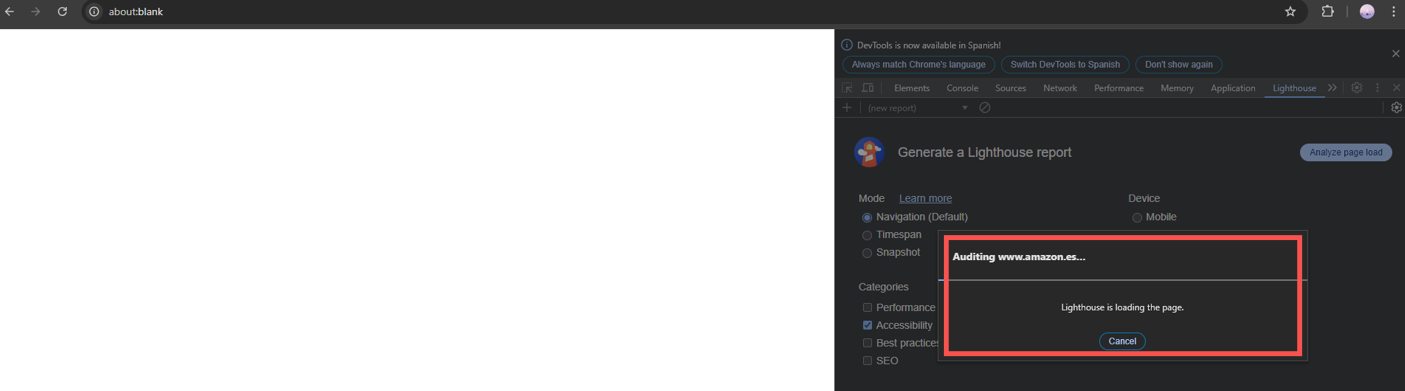
\includegraphics[width=1\textwidth]{figure22.png}
\caption{Mensaje indicador de proceso de análisis.}
\label{fig:22}
\end{figure}

Y nos dará el resultado del análisis de accesibilidad (Figura \ref{fig:23}).

\begin{figure}[H]
\centering
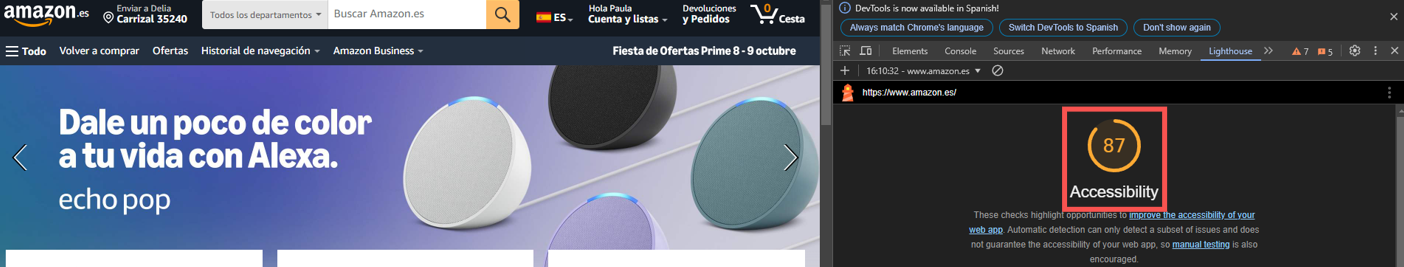
\includegraphics[width=1\textwidth]{figure23.png}
\caption{Resultado del análisis de accesibilidad.}
\label{fig:23}
\end{figure}

El resultado general para Amazon España es una calificación del 87\% de accesibilidad, lo cual es un buen resultado, pero indica que todavía hay margen de mejora. Entre los errores detectados por Lighthouse, se incluyen algunos relacionados con texto alternativo ausente, problemas con el enfoque de los elementos al navegar con teclado, y bajos contrastes en algunas áreas del sitio. Estos problemas se ilustran en las Figuras \ref{fig:23} y \ref{fig:24}, donde se detallan los errores que afectan la accesibilidad de la página.

\begin{figure}[H]
\centering
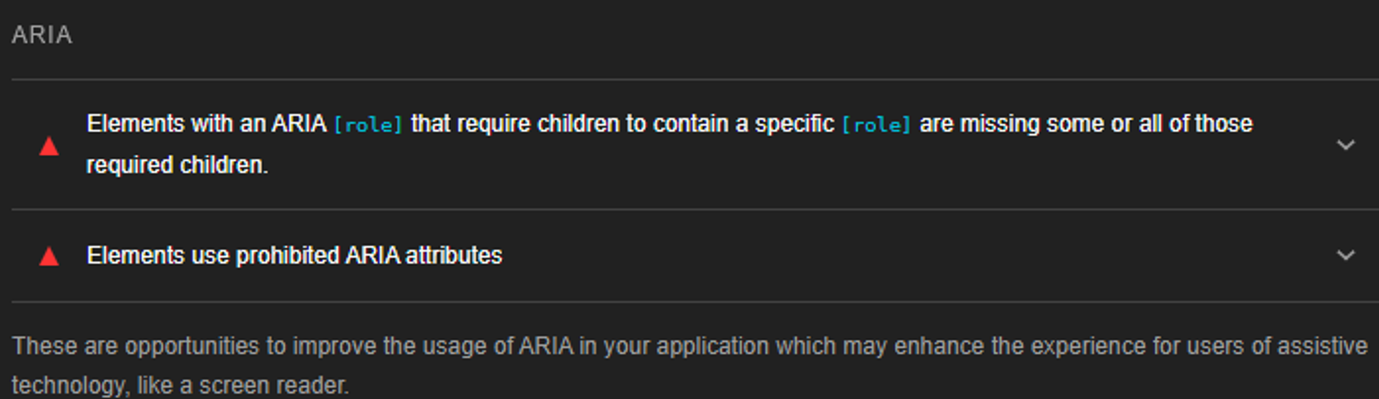
\includegraphics[width=1\textwidth]{figure24.png}
\caption{Errores de accesibilidad en amazon.es según lighthouse.}
\label{fig:24}
\end{figure}

\begin{figure}[H]
\centering
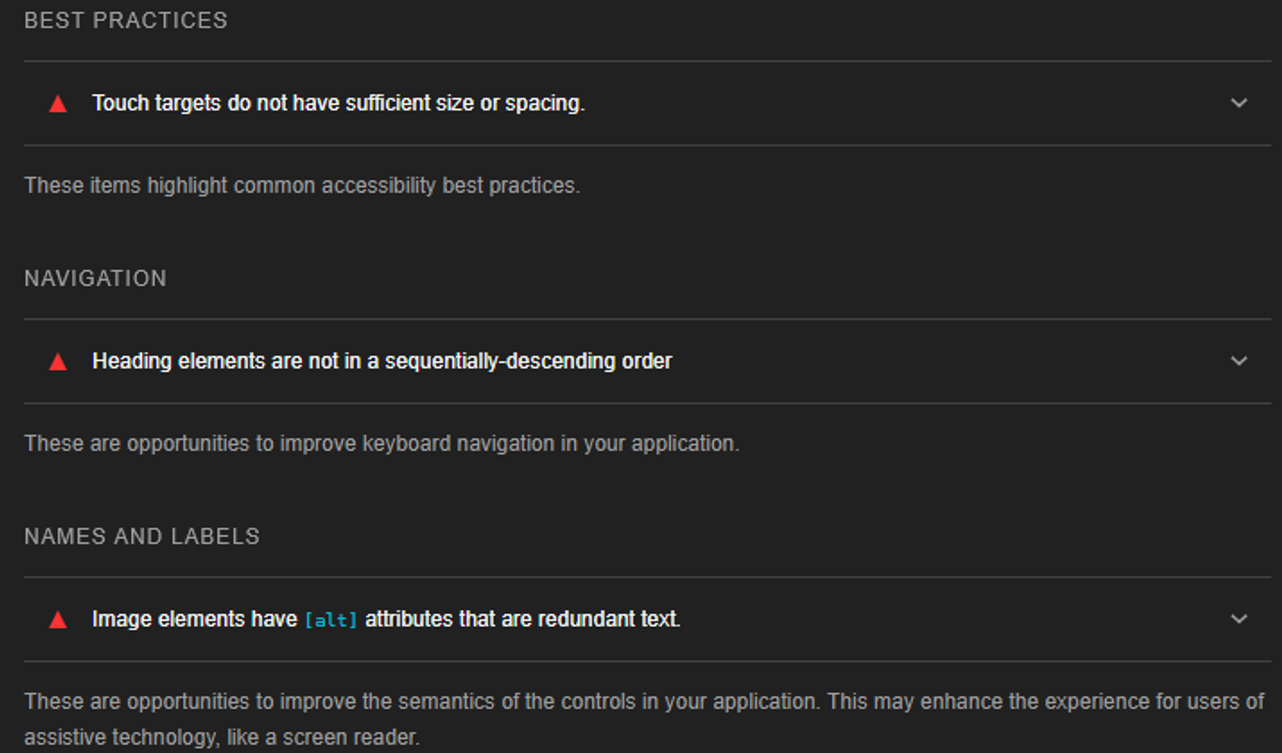
\includegraphics[width=1\textwidth]{figure25.png}
\caption{Errores de accesibilidad en amazon.es según lighthouse.}
\label{fig:25}
\end{figure}

\subsection{Conclusiones del Ejercicio 1}

Al final de este ejercicio, podemos concluir que, si bien Amazon España cumple con muchos de los requisitos de accesibilidad establecidos por las pautas WCAG, existen varias áreas que necesitan mejoras. Los principales problemas detectados afectan a los usuarios que dependen de tecnologías de asistencia como los lectores de pantalla y aquellos que requieren navegación por teclado. Corregir estos errores, así como mejorar los contrastes visuales y la estructura jerárquica de los encabezados, mejoraría significativamente la accesibilidad de la página.

\section{Evaluación de la accesibilidad de la aplicación móvil de Spotify}

Para este segundo ejercicio, seleccionamos una aplicación móvil y evaluamos su accesibilidad siguiendo los principios de las pautas WCAG. En este caso, hemos decidido realizar la evaluación sobre la aplicación móvil de Spotify, basándonos en los cuatro principios fundamentales de las pautas WCAG: Perceptible, Operable, Comprensible y Robustez.

\subsection{Perceptibilidad}

El primer principio para evaluar es la perceptibilidad. Para realizar este análisis, activé el lector de pantalla para Android, TalkBack, que lee en voz alta los elementos presentes en la pantalla, permitiendo a los usuarios navegar la aplicación sin la necesidad de utilizar la vista.

Al activar TalkBack, como se muestra en la Figura \ref{fig:25}, comencé a navegar por la aplicación para observar si el contenido y los elementos de la interfaz eran interpretados correctamente por el lector de pantalla. Durante esta revisión, observé que algunos elementos de la interfaz de Spotify, como las listas de reproducción y los mixes de canciones generados automáticamente, fueron correctamente interpretados por TalkBack, tal y como se muestra en la Figura \ref{fig:26}.

\begin{figure}[H]
\centering
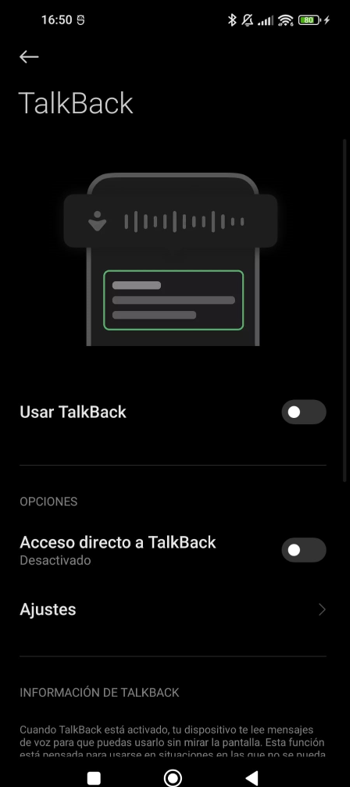
\includegraphics[width=0.5\textwidth]{figure26.png}
\caption{Activación de TalkBack en dispositivo Android.}
\label{fig:26}
\end{figure}


Sin embargo, no todos los elementos de la aplicación son igualmente perceptibles a través del lector de pantalla. Un claro ejemplo de esto es el botón de ajustes que aparece en la interfaz principal. En lugar de proporcionar una descripción adecuada, TalkBack lo lee como "sin texto, botón fuera de la cuadrícula". Esto es un problema importante, ya que los usuarios que dependen del lector de pantalla no podrán comprender la función de este botón y, por lo tanto, se verán limitados en su capacidad para ajustar configuraciones importantes dentro de la aplicación.

\begin{figure}[H]
\centering
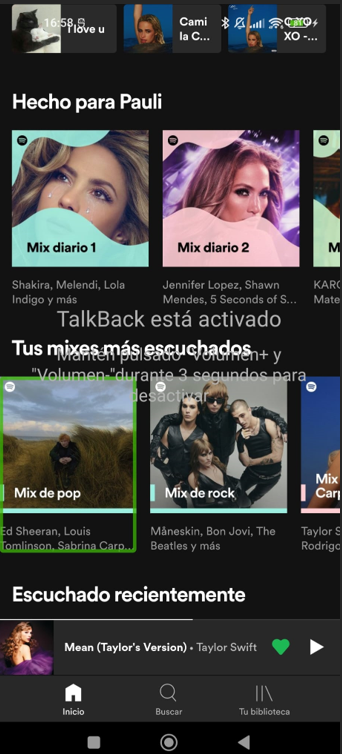
\includegraphics[width=0.5\textwidth]{figure27.png}
\caption{Mix generado por Spotify y con correcta interpretación por parte del lector de pantalla.}
\label{fig:27}
\end{figure}

\begin{figure}[H]
\centering
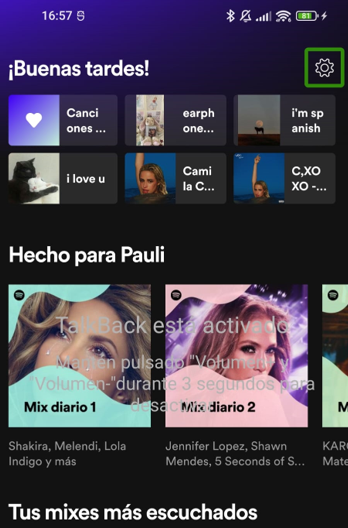
\includegraphics[width=0.6\textwidth]{figure28.png}
\caption{Icono de ajustes el cual no dispone de interpretación por parte del lector de pantalla.}
\label{fig:28}
\end{figure}

Otro aspecto similar ocurre con otros botones importantes, como el de reproducir o el de añadir a favoritos. Estos botones carecen de descripciones precisas y útiles, lo que hace que TalkBack los lea de manera genérica, dificultando a los usuarios la correcta comprensión de sus funciones.

Por otro lado, en términos de contenido visual como imágenes o íconos, Spotify ofrece una buena experiencia en cuanto a contraste y legibilidad. La aplicación utiliza altos contrastes de color, generalmente entre negro y blanco, o verde y blanco, lo que asegura que el contenido sea fácil de distinguir para la mayoría de los usuarios.

\subsection{Operabilidad}

El siguiente principio que evaluar es la operabilidad. Uno de los puntos de este principio es asegurarse de que los objetos táctiles de la interfaz (como botones, íconos y áreas interactivas) tengan un tamaño adecuado. En el caso de Spotify, se observa que los objetos táctiles cumplen con el tamaño mínimo recomendado de 48x48 dp, como lo indican las pautas de diseño de accesibilidad. Este tamaño garantiza que los usuarios, incluyendo aquellos con discapacidades motrices, puedan tocar y seleccionar los elementos correctamente, minimizando el riesgo de errores o de tocar elementos no deseados debido a la proximidad de estos.

Además, Spotify se adapta a las opciones de corrección de color que ofrecen los dispositivos Android en los ajustes de accesibilidad, como se muestra en la Figura \ref{fig:28}.

\begin{figure}[H]
\centering
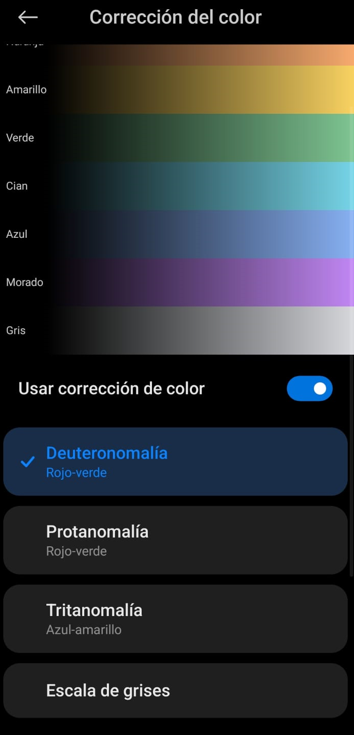
\includegraphics[width=0.5\textwidth]{figure29.png}
\caption{Opciones de corrección de color a las que Spotify es capaz de adaptarse.}
\label{fig:29}
\end{figure}

También está disponible el modo de alto contraste.

Otro aspecto importante es la adaptación al tamaño del texto. Observamos que la interfaz de Spotify responde adecuadamente cuando se cambia el tamaño del texto en las configuraciones del sistema operativo. Cuando el tamaño del texto aumenta, la aplicación ajusta automáticamente la interfaz para mantener todo el contenido legible y organizado, sin que los elementos se superpongan o se pierdan.

\begin{figure}[H]
\centering
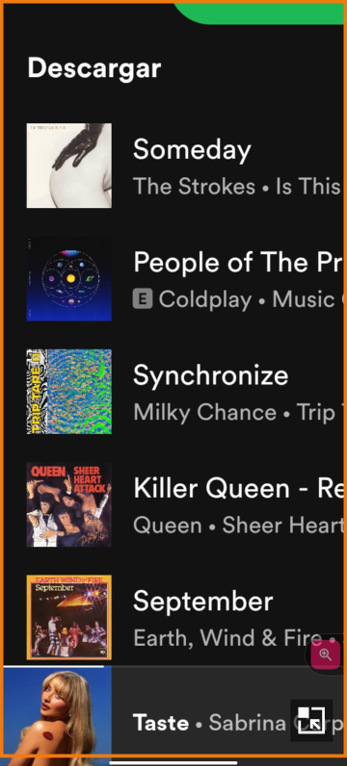
\includegraphics[width=0.5\textwidth]{figure30.png}
\caption{Tamaño de texto ampliado.}
\label{fig:30}
\end{figure}

\subsection{Conclusiones del Ejercicio 2}

Al analizar la accesibilidad de la aplicación móvil de Spotify, observamos varias áreas que cumplen con las pautas WCAG, pero también detectamos deficiencias notables, ya que mientras que muchos elementos, como las listas de reproducción, son correctamente reconocidos por los lectores de pantalla como TalkBack, otros, como algunos botones en la interfaz, carecen de descripciones adecuadas. Esto hace que Spotify avance hacia la accesibilidad, pero necesita mejorar en la correcta etiquetación de todos los elementos interactivos, así como ofrecer mayor soporte para la navegación por teclado y lectores de pantalla para poder  garantizar una experiencia más inclusiva para todos los usuarios.
                   
\end{document}